\documentclass[a4paper]{article}
\usepackage[a4paper]{geometry}
\usepackage{amsmath}
\usepackage{amssymb}
\usepackage[utf8]{inputenc}
\usepackage{graphicx}
\usepackage{booktabs}
\usepackage[russian]{babel}

\title{Лабораторная 2.2.1\\Исследование взаимной диффузии газов}
\date{23 апреля 2017 г.}
\author{Вячеслав Ждановский, студент 611 группы ФРКТ\\
Шамиль Вагабов, студент 611 группы ФРКТ\\
Станислав Токарев, студент 611 группы ФРКТ}
\begin{document}
	\pagenumbering{gobble}
	\maketitle
	\newpage
	\pagenumbering{arabic}
	\paragraph{Цель работы:}
	1) регистрация зависимости концентрации гелия в воздухе от времени с помощью датчиков теплопроводности при разных начальных давлениях смеси газов; 2) определение коэффициента диффузии по результатам измерений.
	\paragraph{В работе используются:}
	измерительная установка; форвакуумный насос; баллон с газом (гелий); манометр; источник питания; магазин сопротивлений; вольметр; ЭВМ
	\paragraph{Теоретические сведения:}
диффузией называют самопроизвольное взаимное проникновение веществ друг в друга, происходящее вследствие хаотичного теплового движения молекул. При перемешивании молекул разного сорта говорят о взаимной (или концентрационной) диффузии. В системе, состоящей из двух компонентов a и b (бинарная смесь), плотности потоков частиц (количество частиц, пересекающих единичную площадку в единицу времени) в результате взаимной диффузии определяются законом Фика:
	 \begin{equation}
	j_a = -D_{ab}\frac{\partial n_a}{\partial x}, \text{ } j_b = -D_{ba}\frac{\partial n_b}{\partial x}
	 \end{equation}
	 где $D$ - коэффициент диффузии, в нашем приближении равный
	 \begin{equation}
	 D=\frac{1}{3}\lambda \bar{v}
	 \end{equation}
	 где $\bar{v}=\sqrt[2]{\frac{8kT}{\pi \mu}}$ - средняя тепловая скорость, $\lambda$ - средняя длина пробега диффундирующих частиц.
	 \begin{equation}
	 \lambda=\frac{1}{n_{\Sigma}\sigma}
	 \end{equation}
	 где $n$ - концентрация, $\sigma$ - среднее сечение столкновения частиц гелия с воздухом.
	 \begin{equation}
	 \implies D \propto \frac{1}{P_{\Sigma}}
	 \end{equation}
	 \paragraph{Схема установки:} 	 
	 Кран К4 обладает повышенной вакуумплотностью и используется для изолирования измерительной части установки от возможных протечек гелия и воздуха. Двухходовой кран К5 служит для подключения форвакуумного насоса к установке, подачи воздуха в установку и соединения форвакуумного насоса с атмосферой. Устройство и назначение кранов К6 и К7 подачи гелия соответствуют основному описанию.\\
	 \begin{figure}[h!]
		\centering
		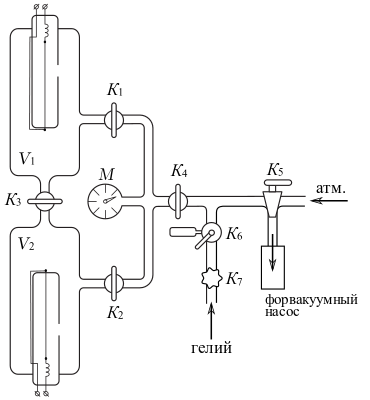
\includegraphics[height=65mm]{pic1.png}
		\caption{Схема установки\label{overflow}}
	 \end{figure}
	   Для исследования взаимной диффузии газов и измерения коэффициента взаимной диффузии D используется  два сосуда  объёмами $V_1$ и $V_2$ ($V_1 \approx V_2 \equiv V$), соединенные трубкой длины L и сечения S (рис. 1). Предполагается, что сосуды заполнены смесью двух газов при одинаковом давлении, но с различной концентрацией компонентов. Вследствие взаимной   диффузии,   проходящей в соединительной трубке, концентрации компонентов в сосудах с течением времени выравниваются. Отметим, что диффузия — относительно медленный процесс, и для его наблюдения необходимо отсутствие конвекции, т.е. макроскопических течений газа как целого. Для этого необходимо обеспечить равенство давлений в сосудах до начала измерений.
	   Путем преобразований получаем:
	 \begin{equation}
	   \Delta n = \Delta n_0 e^{-t/\tau}
	 \end{equation}
	   где $n_0$ - разность концентраций в сосудах в начальный момент.
	   Влиянием силы тяжести пренебрегаем, т.к. $mgh \ll kT$.\\
	   Для измерения разности  концентраций  в установке применяются датчики теплопроводности. При этом используется тот факт, что теплопроводность смеси ($\kappa$) зависит от её состава. В общем случае зависимость $\kappa(n)$ довольно сложна, однако при малой разности  $\Delta n$ концентраций в сосудах можно ожидать, что разность теплопроводностей будет изменяться прямо пропорционально $\Delta n$. \\
	   В процессе диффузии показания вольтметра будут убывать по следующему закону:
	 \begin{equation}
	   U=U_0 e^{-t/\tau}
	 \end{equation}
	 \paragraph{Ход работы:}\text{ }\\
	   1. Включаем все датчики, откачиваем установку, следуя инструкциям. \\
	   2. Выбираем в качестве начального давления - 40 торр.\\
	   3. Изолируем рабочие объемами кранами $K_1$ и $K_2$.\\
	   4. Балансируем мост.\\
	   5. Напускаем гелий и выравниваем давление в сосудах (при этом следим за временем). \\
	   6. Открываем кран $K_3$ и запускаем процесс диффузии.\\
	   7. Берем данные с компьютера. \\
	 8. Повторим измерения для P=80 и 160 торр.\\
	 \begin{figure}[h!]
		\centering
		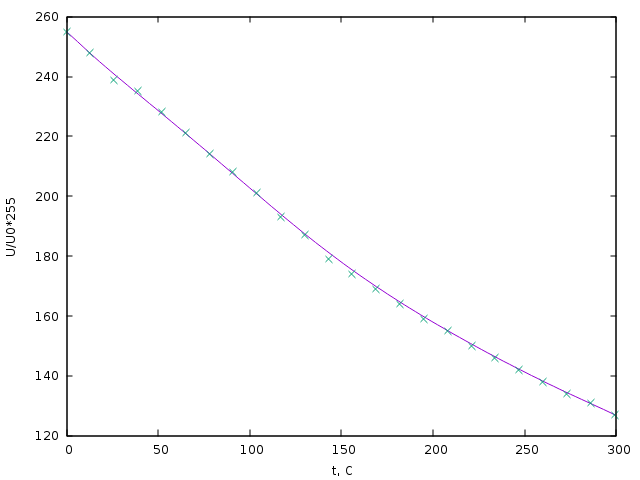
\includegraphics[height=90mm]{plot1.png}
		\caption{P=40 торр\label{overflow}}
	   \end{figure}
	 \begin{figure}[h!]
		\centering
		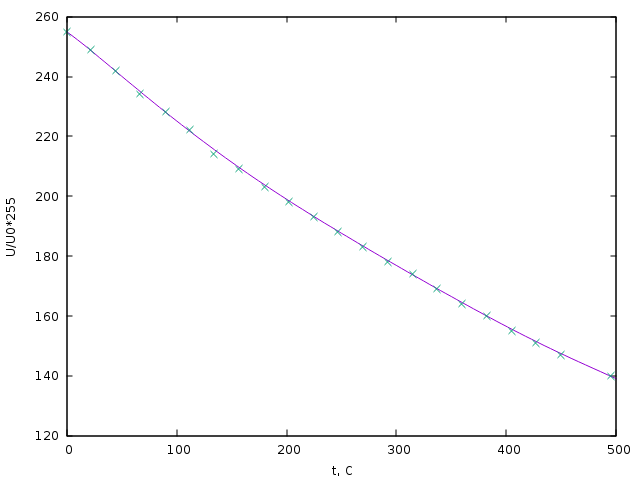
\includegraphics[height=90mm]{plot2.png}
		\caption{P=80 торр\label{overflow}}
	 \end{figure}
	 \begin{figure}[h!]
		\centering
		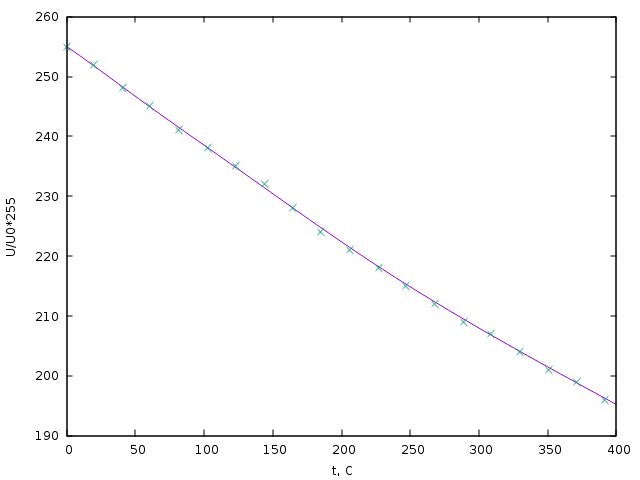
\includegraphics[height=90mm]{plot3.png}
		\caption{P=160 торр\label{overflow}}
	 \end{figure}
	 \begin{table}[h!]
 		\centering
		\begin{tabular}{| c | c | c |}
    		\hline
    		P, торр & D, $\frac{cm^2}{s}$ & $\sigma _D \frac{cm^2}{s}$ \\
    		\hline
    		39.6 & 10,55 & 1.00 \\
    		\hline
    		84 & 5.33 & 4.88 \\
    		\hline
    		162 & 2.95 & 0.27 \\
    		\hline
    	\end{tabular}
  		\caption{Полученные коэффициенты}
	\end{table}\\
	9. Построим график зависимости $D$ от $1/P$.
	\begin{figure}[h!]
		\centering
		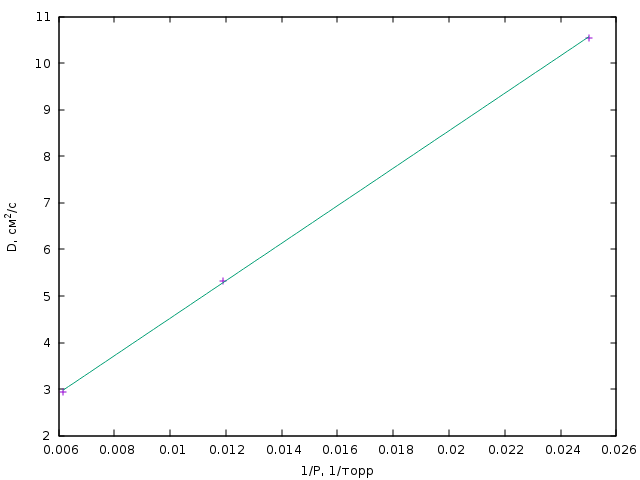
\includegraphics[height=90mm]{plot4.png}
		\caption{Зависимость $D$ от $\frac{1}{P}$\label{overflow}}
	 \end{figure}\\
	 10. Найдем из графика $D$ при $P = 760$ торр.
	 \begin{equation}
	 D=0,55 \pm 0.01 \frac{cm^2}{s}
	 \end{equation}
	 11. Оценим по формулам из теории длину свободного пробега и эффективное сечение столкновения атомов гелия с частицами воздуха.
	 \begin{equation}
	 \lambda_{He} = (137.22 \pm 1.27)\cdot 10^{-9} m
	 \end{equation}
	 \begin{equation}
	 \sigma = (27.12\pm0.25)\cdot 10^{-20} m^2
	 \end{equation}
	 \paragraph{Подведение итогов:}
	 данный метод позволяет максимально полно исследовать явление диффузии газов, экспериментально подтверждая факт того, что к-т диффузии бинарной смеси обратно пропорционален давления и не зависит от пропорций компонентов, а также получать близкие к табличным значения коэффициентов диффузии. 
\end{document}